\chapter{Vector Calculus}

\section{Function ($f(x)$)}

\begin{enumerate}
    \item A function $f$ is a quantity that relates two quantities to each other.
    \hfill \cite{mfml/book/mml/Deisenroth-Faisal-Ong}

    \item These quantities are typically inputs $\bm{x} \in \mbbR^D$ and targets (function values) $f (\bm{x})$, which we assume are real-valued if not stated otherwise.
    \hfill \cite{mfml/book/mml/Deisenroth-Faisal-Ong}

    \item $\mbbR^D$ is the domain of $f$ , and the function values $f (\bm{x})$ are the image/codomain of $f$ .
    \hfill \cite{mfml/book/mml/Deisenroth-Faisal-Ong}

    \item We often write
    \hfill \cite{mfml/book/mml/Deisenroth-Faisal-Ong}
    \begin{enumerate}
        \item $f: \mbbR^D \to \mbbR$
        (specifies that $f$ is a mapping from $\mbbR^D$ to $\mbbR$ )
        \hfill \cite{mfml/book/mml/Deisenroth-Faisal-Ong}

        \item $\bm{x} \mapsto f(\bm{x})$
        (specifies the explicit assignment of an input $\bm{x}$ to a function value $f(\bm{x})$)
        \hfill \cite{mfml/book/mml/Deisenroth-Faisal-Ong}
    \end{enumerate}
    to specify a function.
    \hfill \cite{mfml/book/mml/Deisenroth-Faisal-Ong}

    \item A function $f$ assigns every input x exactly one function value $f (\bm{x})$.
    \hfill \cite{mfml/book/mml/Deisenroth-Faisal-Ong}
\end{enumerate}

\vspace{0.5cm}
\textbf{ALSO SEE/ RELATED}:
\begin{enumerate}
    \item \fullref{vector space/Linear Mappings}
\end{enumerate}



\subsection{Differentiation of Uni-variate Functions}

\begin{enumerate}
    \item
    \begin{definition}[Univariate function ($f : \mbbR \to \mbbR$)]
        Univariate function: $y = f(x),\ x, y \in \mbbR$
        \hfill \cite{mfml/book/mml/Deisenroth-Faisal-Ong}
    \end{definition}

    \item
    \begin{definition}[Difference Quotient]
        The difference quotient
        $
            \dfrac{\delta y}{\delta x}
            := \dfrac{f(x + \delta x) - f(x)}{\delta x}
        $
        computes the slope of the secant line through two points on the graph of $f$ .
        \hfill \cite{mfml/book/mml/Deisenroth-Faisal-Ong}
    \end{definition}

    \item The derivative of $f$ points in the direction of steepest ascent of $f$.
    \hfill \cite{mfml/book/mml/Deisenroth-Faisal-Ong}

    \item
    \begin{definition}[Power Series]
        $
            f(x) = \dsum_{k=0}^{\infty} a_k (x-c)^k
        $
        \\
        where $a_k$ are coefficients and $c$ is a constant
    \end{definition}

\end{enumerate}




\subsection{Differentiation of multi-variate Functions}

\begin{enumerate}
    \item
    \begin{definition}[multi-variate Functions ($f : \mbbR^n \to \mbbR$)]
        The general case where the function $f$ depends on one or more variables $\bm{x} \in \mbbR^n$
        \hfill \cite{mfml/book/mml/Deisenroth-Faisal-Ong}
    \end{definition}

    \item
    \begin{definition}[Partial Derivative ($\dfrac{\partial f}{\partial x_i}$)]
        For a function $f : \mbbR^n \to \mbbR$, $\bm{x} \mapsto f (\bm{x})$, $\bm{x} \in \mbbR^n$ of $n$ variables $x_1, \cdots , x_n$ we define the partial derivatives as
        \hfill \cite{mfml/book/mml/Deisenroth-Faisal-Ong}
        \\
        .\hfill
        ${
            \displaystyle
            \begin{matrix}
                \dfrac{\partial f}{\partial x_1}
                &
                =
                &
                \lim_{h\to 0} \dfrac{f (x_1 + h, x_2, \cdots , x_n) - f (\bm{x})}{h}
                \\
                & \vdots &
                \\
                \dfrac{\partial f}{\partial x_n}
                &
                =
                &
                \lim_{h\to 0} \dfrac{f (x_1 , x_2, \cdots , x_n+ h) - f (\bm{x})}{h}
            \end{matrix}
        }$
        \hfill \cite{mfml/book/mml/Deisenroth-Faisal-Ong}
    \end{definition}
\end{enumerate}

\subsubsection{Gradient}

\begin{enumerate}
    \item The generalization of the derivative to functions of several variables is the \textbf{gradient}.
    \hfill \cite{mfml/book/mml/Deisenroth-Faisal-Ong}

    \item We find the gradient of the function $f$ with respect to $\bm{x}$ by varying one variable at a time and keeping the others constant.
    \hfill \cite{mfml/book/mml/Deisenroth-Faisal-Ong}

    \item The gradient is then the \textbf{collection} of these partial derivatives.
    \hfill \cite{mfml/book/mml/Deisenroth-Faisal-Ong}

    \item
    \begin{definition}[Gradient ($\nabla_x f \in \mbbR^{1 \times n}$)]
        For a function $f : \mbbR^n \to \mbbR$, $\bm{x} \mapsto f (\bm{x})$, $\bm{x} \in \mbbR^n$ of $n$ variables $x_1, \cdots , x_n$:
        \\
        .\hfill
        $
            \nabla_x f
            = \text{grad} f
            = \dfrac{df}{d\bm{x}}
            = \begin{bmatrix}
                \dfrac{\partial f(\bm{x})}{\partial x_1} &
                \dfrac{\partial f(\bm{x})}{\partial x_2} &
                \cdots
                \dfrac{\partial f(\bm{x})}{\partial x_n}
            \end{bmatrix}
            \in \mbbR^{1 \times n}
        $
        \hfill \cite{mfml/book/mml/Deisenroth-Faisal-Ong}
        \\
        where $n$ is the number of variables and $1$ is the dimension of the image/range/codomain of $f$ .
        The row vector is called the gradient of $f$ or the Jacobian.
        \hfill \cite{mfml/book/mml/Deisenroth-Faisal-Ong}
    \end{definition}

    \item This definition of Jacobian is a special case of the general definition of the Jacobian for vector-valued functions as the collection of partial derivatives.
    \hfill \cite{mfml/book/mml/Deisenroth-Faisal-Ong}

    \item The reason why we define the gradient vector as a row vector:
    \hfill \cite{mfml/book/mml/Deisenroth-Faisal-Ong}
    \begin{enumerate}
        \item we can consistently generalize the gradient to vector-valued functions $f : \mbbR^n \to \mbbR^m$ (then the gradient becomes a matrix)
        \hfill \cite{mfml/book/mml/Deisenroth-Faisal-Ong}

        \item we can immediately apply the multi-variate chain rule without paying attention to the dimension of the gradient.
        \hfill \cite{mfml/book/mml/Deisenroth-Faisal-Ong}
    \end{enumerate}
\end{enumerate}






\section{Gradients of Vector-Valued Functions ($J = \nabla_x f$)}

\begin{enumerate}
    \item
    \begin{definition}[vector-valued functions/ vector fields ($\bm{f} : \mbbR^n \to \mbbR^m$)]
        vector-valued functions (vector fields) are defined as $\bm{f} : \mbbR^n \to \mbbR^m$, where $n \geq 1$ and $m > 1$.
        For a function $\bm{f} : \mbbR^n \to \mbbR^m$ and a vector $\bm{x} = [x_1, \cdots , x_n]^\top \in \mbbR^n$, the corresponding vector of function values is given as
        $
            \bm{f}(\bm{x})
            = \begin{bmatrix}
                f_1(\bm{x}) \\
                \vdots \\
                f_m(\bm{x})
            \end{bmatrix}
            \in \mbbR^m
        $
        \hfill \cite{mfml/book/mml/Deisenroth-Faisal-Ong}
    \end{definition}

    \item Writing the vector-valued function in this way allows us to view a vector-valued function $\bm{f} : \mbbR^n \to \mbbR^m$ as a vector of functions $[f_1, \cdots , f_m]^\top$, $f_i : \mbbR^n \to \mbbR$ that map onto $\mbbR$.
    \hfill \cite{mfml/book/mml/Deisenroth-Faisal-Ong}

    \item
    .\hfill
    ${
        \displaystyle
        \dfrac{\partial\bm{f}}{\partial x_i}
        = \begin{bmatrix}
            \dfrac{\partial f_1}{\partial x_i} \\
            \vdots \\
            \dfrac{\partial f_m}{\partial x_i}
        \end{bmatrix}
        = \begin{bmatrix}
            \lim_{h \to 0} \dfrac{f_1(x_1,\cdots,x_{i-1},x_i+h,x_{i+1},\cdots x_n)-f_1(\bm{x})}{h} \\
            \vdots \\
            \lim_{h \to 0} \dfrac{f_m(x_1,\cdots,x_{i-1},x_i+h,x_{i+1},\cdots x_n)-f_m(\bm{x})}{h}
        \end{bmatrix}
        \in \mbbR^m
    }$
    \hfill \cite{mfml/book/mml/Deisenroth-Faisal-Ong}

    \item
    \begin{definition}[Jacobian ($\bm{J} = \nabla_{\bm{x}}\bm{f} = \dfrac{d \bm{f}(\bm{x})}{d \bm{x}}$)]
        The collection of all first-order partial derivatives of a vector-valued function $\bm{f} : \mbbR^n \to \mbbR^m$ is called the Jacobian.
        The Jacobian $\bm{J}$ is an $m \times n$ matrix, which we define and arrange as follows:
        \hfill \cite{mfml/book/mml/Deisenroth-Faisal-Ong}
        \\
        .\hfill
        $
            \bm{J}
            = \nabla_{\bm{x}}\bm{f}
            = \dfrac{d \bm{f}(\bm{x})}{d \bm{x}}
            = \begin{bmatrix}
                \dfrac{\partial \bm{f}(\bm{x})}{\partial x_1} &
                \cdots &
                \dfrac{\partial \bm{f}(\bm{x})}{\partial x_n}
            \end{bmatrix}
            = \begin{bmatrix}
                \dfrac{\partial f_1(\bm{x})}{\partial x_1} &
                \cdots &
                \dfrac{\partial f_1(\bm{x})}{\partial x_n} \\
                \vdots & \ddots & \vdots \\
                \dfrac{\partial f_m(\bm{x})}{\partial x_1} &
                \cdots &
                \dfrac{\partial f_m(\bm{x})}{\partial x_n} \\
            \end{bmatrix}
            \in \mbbR^{m\times n}
        $
        \hfill \cite{mfml/book/mml/Deisenroth-Faisal-Ong}
        \\
        .\hfill
        $
            \bm{x} = \begin{bmatrix}
                x_1 \\ \cdots \\ x_n
            \end{bmatrix},
            \hspace{1cm}
            J(i,j) = \dfrac{\partial f_i}{\partial x_j}
        $
        \hfill \cite{mfml/book/mml/Deisenroth-Faisal-Ong}
    \end{definition}
    \begin{enumerate}
        \item As a special case, a function $f : \mbbR^n \to \mbbR^1$, which maps a vector $\bm{x} \in \mbbR^n$ onto a scalar (e.g., $f (x) = \dsum^n _{i=1} x_i$), possesses a Jacobian that is a row vector (matrix of dimension $1 \times n$)
        \hfill \cite{mfml/book/mml/Deisenroth-Faisal-Ong}

        \item Jacobian is used in the change-of-variable method for probability distributions.
        The amount of scaling due to the transformation of a variable is provided by the determinant.
        \hfill \cite{mfml/book/mml/Deisenroth-Faisal-Ong}

        \item The absolute value of the Jacobian determinant $\dabs{det(\bm{J})}$ is the factor by which areas or volumes are scaled when coordinates are transformed.
        \hfill \cite{mfml/book/mml/Deisenroth-Faisal-Ong}

        \item Geometrically, the Jacobian determinant gives the magnification/ scaling factor when we transform an area or volume.
        \hfill \cite{mfml/book/mml/Deisenroth-Faisal-Ong}
    \end{enumerate}

\end{enumerate}







\section{Higher-Order Derivatives}

.\hfill
$
    \dfrac{\partial^2 f}{\partial x^2} = \dfrac{\partial}{\partial x} \dParenBrac{\dfrac{\partial f}{\partial x}}
$
\hfill \vrule \hfill
$
    \dfrac{\partial^2 f}{\partial y \partial x} = \dfrac{\partial}{\partial y} \dParenBrac{\dfrac{\partial f}{\partial x}}
$
\hfill \vrule \hfill
$
    \dfrac{\partial^2 f}{\partial x \partial y} = \dfrac{\partial}{\partial x} \dParenBrac{\dfrac{\partial f}{\partial y}}
$
\hfill \cite{mfml/book/mml/Deisenroth-Faisal-Ong}
\\[0.2cm]
.\hfill
$
    \dfrac{\partial^n f}{\partial x^n} =
    \dfrac{\partial}{\partial x} \dParenBrac{
        \overset{n \text{ times}}{\cdots}
        \dParenBrac{\dfrac{\partial}{\partial x} \dParenBrac{\dfrac{\partial f}{\partial x}}}
        \cdots
    }
$
\hfill \cite{mfml/book/mml/Deisenroth-Faisal-Ong}

\begin{enumerate}
    \item
    \begin{definition}[Hessian ($\bm{H} = \nabla^2_{x,y}f(x,y)$)]
        The Hessian is the collection of all second-order partial derivatives.
        \hfill \cite{mfml/book/mml/Deisenroth-Faisal-Ong}
    \end{definition}

    \item If $f (x, y)$ is a twice (continuously) differentiable function, then
    $
        \dfrac{\partial^2 f}{\partial y \partial x}
        = \dfrac{\partial^2 f}{\partial x \partial y}
    $
    \hfill \cite{mfml/book/mml/Deisenroth-Faisal-Ong}

    \item
    $
        \bm{H}
        = \nabla^2_{x,y}f(x,y)
        = \begin{bmatrix}
            \dfrac{\partial^2 f}{\partial x^2} & \dfrac{\partial^2 f}{\partial x \partial y} \\
            \dfrac{\partial^2 f}{\partial x \partial y} & \dfrac{\partial^2 f}{\partial y^2}
        \end{bmatrix}
    $
    \hfill \cite{mfml/book/mml/Deisenroth-Faisal-Ong}

    \item Generally, for $\bm{x} \in \mbbR^n$ and $f : \mbbR^n \to \mbbR$, the Hessian is an $n \times n$ matrix.
    The Hessian measures the curvature of the function locally around $(x, y)$.
    \hfill \cite{mfml/book/mml/Deisenroth-Faisal-Ong}

    \item (Hessian of a Vector Field) If $\bm{f} : \mbbR^n \to \mbbR^m$ is a vector field, the Hessian is an $(m \times n \times n)$-tensor.
    \hfill \cite{mfml/book/mml/Deisenroth-Faisal-Ong}
\end{enumerate}














\section{Gradients of Matrices}


\begin{table}[H]
\hfill
\begin{minipage}{0.45\linewidth}
\begin{figure}[H]
    \centering
    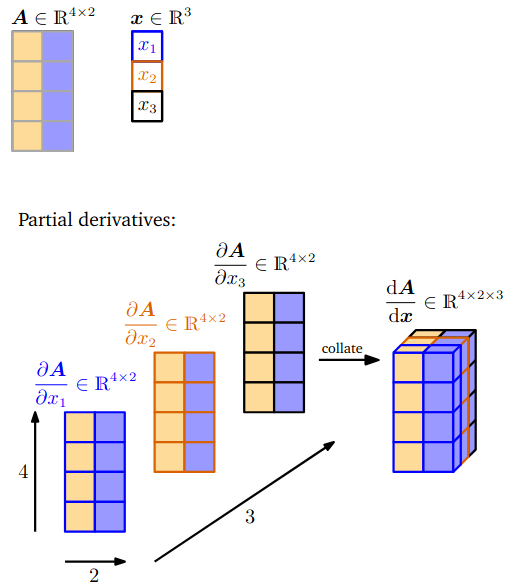
\includegraphics[
        width=\linewidth,
        height=5cm,
        keepaspectratio,
    ]{images/Vector-Calculus/Gradients-of-Matrices-approach1.png}
    \caption*{
        \textbf{Approach 1}:
        We compute the partial derivative
        $\dfrac{\partial \bm{A}}{\partial x_1}$ ,
        $\dfrac{\partial \bm{A}}{\partial x_2}$ ,
        $\dfrac{\partial \bm{A}}{\partial x_3}$ , each of which is a $4 \times 2$ matrix,
        and collate them in a $4 \times 2 \times 3$ tensor.
        \cite{mfml/book/mml/Deisenroth-Faisal-Ong}
    }
\end{figure}
\end{minipage}
\hfill
\begin{minipage}{0.45\linewidth}
\begin{figure}[H]
    \centering
    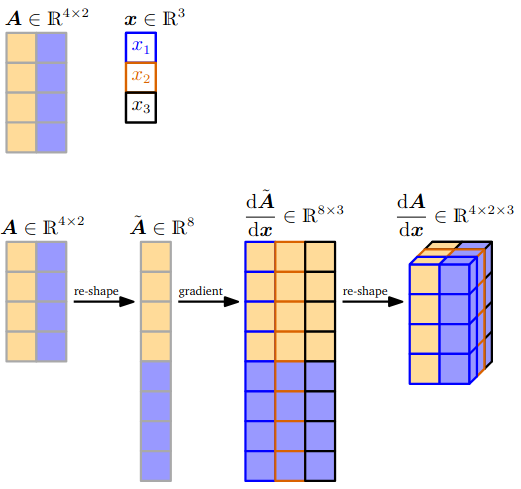
\includegraphics[
        width=\linewidth,
        height=5cm,
        keepaspectratio,
    ]{images/Vector-Calculus/Gradients-of-Matrices-approach2.png}
    \caption*{
        \textbf{Approach 2}: We re-shape (flatten) $\bm{A} \in \mbbR^{4\times 2}$ into a vector $\tilde{\bm{A}} \in \mbbR^8$.
        Then, we compute the gradient $\dfrac{d\tilde{\bm{A}}}{d\bm{x}} \in \mbbR^{8\times 3}$.
        We obtain the gradient tensor by re-shaping this gradient as illustrated above.
        \cite{mfml/book/mml/Deisenroth-Faisal-Ong}
    }
\end{figure}
\end{minipage}
\hfill
\end{table}


\begin{enumerate}
    \item
    \begin{definition}[Tensor]
        Tensor is a multidimensional array
        \hfill \cite{mfml/book/mml/Deisenroth-Faisal-Ong}
    \end{definition}

    \item
    \begin{definition}[Flattening (matrix $\to$ vector)]
        Matrices can be transformed into vectors by stacking the columns of the matrix
        \hfill \cite{mfml/book/mml/Deisenroth-Faisal-Ong}
    \end{definition}

    \item if we compute the gradient of an $m \times  n$ matrix $\bm{A}$ with respect to a $p \times  q$ matrix $\bm{B}$, the resulting Jacobian would be $(m\times n)\times (p\times q)$, i.e., a four-dimensional tensor $\bm{J}$, whose entries are given as $J_{ijkl} = \dfrac{\partial A_{ij}}{\partial B_{kl}}$.
    \hfill \cite{mfml/book/mml/Deisenroth-Faisal-Ong}
\end{enumerate}










\section{Differentiation Rules}

\begin{enumerate}[series=vcalrules]
    \item \textbf{Product rule}:
    \begin{enumerate}
        \item $
            (f(x)g(x))^\prime
            = \dfrac{d}{dx}(f(x)g(x))
            = g(x)\dfrac{d}{dx}f(x) + f(x)\dfrac{d}{dx}g(x)
            = f^\prime(x)g(x) + f(x)g^\prime(x)
        $
        \hfill \cite{mfml/book/mml/Deisenroth-Faisal-Ong}

        \item $
            \dfrac{\partial}{\partial \bm{x}}(f(\bm{x})g(\bm{x}))
            = g(\bm{x})\dfrac{\partial}{\partial \bm{x}}f(\bm{x})
                + f(\bm{x})\dfrac{\partial}{\partial \bm{x}}g(\bm{x})
        $ \hfill \cite{mfml/book/mml/Deisenroth-Faisal-Ong}
    \end{enumerate}

    \item \textbf{Quotient rule}:
    $
        \dParenBrac{\dfrac{f(x)}{g(x)}}^\prime
        = \dfrac{d}{dx}\dParenBrac{\dfrac{f(x)}{g(x)}}
        = \dfrac{f^\prime(x)g(x) - f(x)g^\prime(x)}{(g(x))^2}
    $
    \hfill \cite{mfml/book/mml/Deisenroth-Faisal-Ong}

    \item \textbf{Sum Rule}:
    \begin{enumerate}
        \item $
            (f(x) + g(x))^\prime
            = f^\prime(x) + g^\prime(x)
        $
        \hfill \cite{mfml/book/mml/Deisenroth-Faisal-Ong}

        \item $
            \dfrac{\partial}{\partial \bm{x}}(f(\bm{x}) + g(\bm{x}))
            = \dfrac{\partial}{\partial \bm{x}}f(\bm{x})
                + \dfrac{\partial}{\partial \bm{x}}g(\bm{x})
        $
        \hfill \cite{mfml/book/mml/Deisenroth-Faisal-Ong}
    \end{enumerate}

    \item \textbf{Chain Rule}:
    \begin{enumerate}
        \item $
            (g(f(x)))^\prime
            = (g \circ f)^\prime(x)
            = g^\prime(f(x)) f^\prime(x)
        $
        \hfill \cite{mfml/book/mml/Deisenroth-Faisal-Ong}

        \item $
            \dfrac{\partial}{\partial \bm{x}}(g(f(\bm{x})))
            = \dfrac{\partial}{\partial \bm{x}}(g \circ f)(\bm{x})
            = \dfrac{\partial g(\bm{x})}{\partial f(\bm{x})}
                \dfrac{\partial f(\bm{x})}{\partial \bm{x}}
        $
        \hfill \cite{mfml/book/mml/Deisenroth-Faisal-Ong}
    \end{enumerate}
    $g \circ f$ denotes function composition $x \mapsto f (x) \mapsto g(f (x))$.
    \hfill \cite{mfml/book/mml/Deisenroth-Faisal-Ong}
\end{enumerate}

\vspace{0.5cm}
\textbf{Gradients of Matrices \& Vectors}:

\begin{multicols}{2}
\begin{enumerate}[resume*=vcalrules]
    \item $
        \dfrac{\partial \bm{f}(\bm{A})^\top}{\partial \bm{A}}
        = \dParenBrac{\dfrac{\partial \bm{f}(\bm{A})}{\partial \bm{A}}}^\top
    $
    \hfill \cite{mfml/book/mml/Deisenroth-Faisal-Ong}

    \item $
        \dfrac{\partial\ \tr(\bm{f}(\bm{A}))}{\partial \bm{A}}
        = \tr\dParenBrac{\dfrac{\partial \bm{f}(\bm{A})}{\partial \bm{A}}}
    $
    \hfill \cite{mfml/book/mml/Deisenroth-Faisal-Ong}

    \item
    $
        \dfrac{\partial \bm{f}(\bm{A})^{-1}}{\partial \bm{A}}
        = -\bm{f}(\bm{A})^{-1}\ \dfrac{\partial \bm{f}(\bm{A})}{\partial \bm{A}} \ \bm{f}(\bm{A})^{-1}
    $
    \hfill \cite{mfml/book/mml/Deisenroth-Faisal-Ong}

    \item
    $
        \dfrac{\partial\ \bm{x}^\top \bm{A}^{-1}\bm{y}}{\partial \bm{A}}
        = -(\bm{A}^{-1})^\top \bm{xy}^\top (\bm{A}^{-1})^\top
    $
    \hfill \cite{mfml/book/mml/Deisenroth-Faisal-Ong}

    \item
    $
        \dfrac{\partial\ \bm{x}^\top \bm{A}\bm{y}}{\partial \bm{A}}
        = \bm{xy}^\top
    $
    \hfill \cite{mfml/book/mml/Deisenroth-Faisal-Ong}

    \item
    $
        \dfrac{\partial\ \bm{x}^\top \bm{A}\bm{x}}{\partial \bm{x}}
        = \bm{x}^\top(\bm{A} + \bm{A}^\top)
    $
    \hfill \cite{mfml/book/mml/Deisenroth-Faisal-Ong}

    \item
    $
        \dfrac{\partial\ \bm{x}^\top \bm{y}}{\partial\ \bm{x}} = \bm{y}^\top
    $
    \hfill \cite{mfml/book/mml/Deisenroth-Faisal-Ong}

    \item
    $
        \dfrac{\partial\ \bm{y}^\top \bm{x}}{\partial\ \bm{x}} = \bm{y}^\top
    $
    \hfill \cite{mfml/book/mml/Deisenroth-Faisal-Ong}
\end{enumerate}
\end{multicols}

\vspace{0.5cm}
\begin{enumerate}[resume*=vcalrules]
    \item $
        \dfrac{\partial \det(\bm{f}(\bm{A}))}{\partial \bm{A}}
        = \det(\bm{f}(\bm{A}))\ \tr\dParenBrac{\bm{f}(\bm{A})^{-1}\ \dfrac{\partial \bm{f}(\bm{A})}{\partial \bm{A}}}
    $
    \hfill \cite{mfml/book/mml/Deisenroth-Faisal-Ong}

    \item
    $
        \dfrac{\partial\ (\bm{x} - \bm{As})^\top \bm{W} (\bm{x} - \bm{As})}{\partial\bm{s}}
        = -2(\bm{x} - \bm{As})^\top \bm{WA}
    $
    \hfill
    (for symmetric $\bm{W}$)
    \hfill \cite{mfml/book/mml/Deisenroth-Faisal-Ong}
\end{enumerate}


\vspace{0.5cm}
\textbf{Examples}
\begin{enumerate}
    \item Consider a function $f : \mbbR^2 \to \mbbR$ of two variables $x_1, x_2$.
    Furthermore, $x_1(t)$ and $x_2(t)$ are themselves functions of $t$.
    \\
    $
        \nabla_t f(x_1, x_2)
        = \dfrac{df}{dt}
        = \begin{bmatrix}
            \dfrac{\partial f(x_1, x_2)}{\partial x_1(t)} &
            \dfrac{\partial f(x_1, x_2)}{\partial x_2(t)}
        \end{bmatrix}
        \begin{bmatrix}
            \dfrac{\partial x_1(t)}{\partial t} \\
            \dfrac{\partial x_2(t)}{\partial t}
        \end{bmatrix}
        = \dfrac{\partial f(x_1, x_2)}{\partial x_1(t)} \dfrac{\partial x_1(t)}{\partial t}
        + \dfrac{\partial f(x_1, x_2)}{\partial x_2(t)} \dfrac{\partial x_2(t)}{\partial t}
    $
    \hfill \cite{mfml/book/mml/Deisenroth-Faisal-Ong}

    \item If $f (x_1, x_2)$ is a function of $x_1$ and $x_2$, where $x_1(s, t)$ and $x_2(s, t)$ are themselves functions of two variables $s$ and $t$:
    \\
    $
        \begin{aligned}
        \nabla_{(s,t)} f(x_1, x_2)
        &= \dfrac{df(x_1, x_2)}{d(s,t)}
        = \dfrac{\partial f}{\partial \bm{x}} \dfrac{\partial \bm{x}}{\partial (s,t)}
        = \begin{bmatrix}
            \dfrac{\partial f(x_1, x_2)}{\textcolor{blue}{\partial x_1(s,t)}} &
            \dfrac{\partial f(x_1, x_2)}{\textcolor{green}{\partial x_2(s,t)}}
        \end{bmatrix}
        \begin{bmatrix}
            \textcolor{blue}{\dfrac{\partial x_1(s,t)}{\partial s}} & \textcolor{blue}{\dfrac{\partial x_1(s,t)}{\partial t}} \\
            \textcolor{green}{\dfrac{\partial x_2(s,t)}{\partial s}} & \textcolor{green}{\dfrac{\partial x_2(s,t)}{\partial t}}
        \end{bmatrix}
        \\
        &=
        \begin{bmatrix}
            \dfrac{\partial f(x_1, x_2)}{\textcolor{blue}{\partial x_1(s,t)}}
            \textcolor{blue}{\dfrac{\partial x_1(s,t)}{\partial s}} +
            \dfrac{\partial f(x_1, x_2)}{\textcolor{green}{\partial x_2(s,t)}}
            \textcolor{green}{\dfrac{\partial x_2(s,t)}{\partial s}} \\
            \dfrac{\partial f(x_1, x_2)}{\textcolor{blue}{\partial x_1(s,t)}}
            \textcolor{blue}{\dfrac{\partial x_1(s,t)}{\partial t}} +
            \dfrac{\partial f(x_1, x_2)}{\textcolor{green}{\partial x_2(s,t)}}
            \textcolor{green}{\dfrac{\partial x_2(s,t)}{\partial t}}
        \end{bmatrix}
        \end{aligned}
    $
    \hfill \cite{mfml/book/mml/Deisenroth-Faisal-Ong}

\end{enumerate}




















\section{Backpropagation: Gradients in DNN}

\begin{table}[H]
\begin{minipage}{0.48\linewidth}
    \begin{figure}[H]
        \centering
        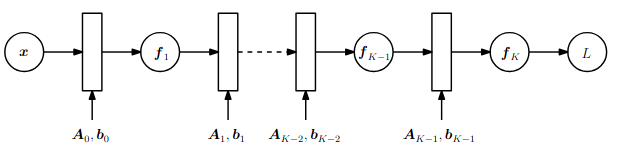
\includegraphics[
            width=\linewidth,
            height=3cm,
            keepaspectratio,
        ]{images/Vector-Calculus/sample-dnn-bp-ad.png}
        \caption*{
            Forward pass in a multi-layer neural network to compute the loss $L$ as a function of the inputs $\bm{x}$ and the parameters $\bm{A}_i, \bm{b}_i$.
            \cite{mfml/book/mml/Deisenroth-Faisal-Ong}
        }
    \end{figure}
\end{minipage}
\hfill
\vline
\hfill
\begin{minipage}{0.48\linewidth}
    \begin{figure}[H]
        \centering
        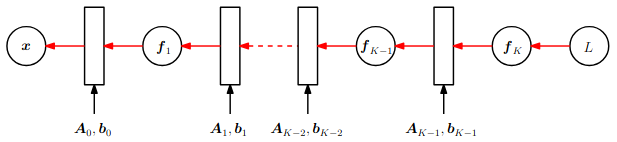
\includegraphics[
            width=\linewidth,
            height=3cm,
            keepaspectratio,
        ]{images/Vector-Calculus/sample-dnn-bp-ad2.png}
        \caption*{
            Backward pass in a multi-layer neural network to compute the gradients of the loss function.
            \cite{mfml/book/mml/Deisenroth-Faisal-Ong}
        }
    \end{figure}
\end{minipage}
\end{table}

\begin{enumerate}
    \item An area where the chain rule is used to an extreme is deep learning, where the function value $\bm{y}$ is computed as a many-level function composition
    \hfill \cite{mfml/book/mml/Deisenroth-Faisal-Ong}
    \\
    .\hfill
    $
        \bm{y}
        = (f_K \circ f_{K-1} \circ \cdots \circ f_1)(\bm{x})
        = f_K (f_{K-1}(\cdots (f_1(\bm{x}))\cdots))
    $
    \hfill \cite{mfml/book/mml/Deisenroth-Faisal-Ong}
    \\
    where $\bm{x}$ are the inputs (e.g., images), $\bm{y}$ are the observations (e.g., class labels), and every function $f_i, i = 1, \cdots , K$, possesses its own parameters.
    \hfill \cite{mfml/book/mml/Deisenroth-Faisal-Ong}
    \\
    \begin{multicols}{2}
    \begin{enumerate}[series=grad-dnn]
        \item $\bm{f}_0 := \bm{x}$
        \hfill \cite{mfml/book/mml/Deisenroth-Faisal-Ong}

        \item $\bm{f}_i := \sigma_i(\bm{A}_{i-1}\bm{f}_{i-1} + \bm{b}_{i-1})$
        \hfill \cite{mfml/book/mml/Deisenroth-Faisal-Ong}

        \item $\bm{f}_i(\bm{x}_{i-1}) = \sigma_i(\bm{A}_{i-1}\bm{x}_{i-1} + \bm{b}_{i-1})$
        \hfill \cite{mfml/book/mml/Deisenroth-Faisal-Ong}

        \item $\bm{y} = \bm{f}_K(\bm{x}_{K-1})$
        \hfill \cite{mfml/book/mml/Deisenroth-Faisal-Ong}
    \end{enumerate}
    \end{multicols}
    \begin{multicols}{2}
    \begin{enumerate}[resume*=grad-dnn]
        \item $L(\bm{\theta}) = \dnorm{\bm{y} - \bm{f}_K(\bm{\theta},\ \bm{x})}^2$
        \hfill \cite{mfml/book/mml/Deisenroth-Faisal-Ong}

        \item
        $
            \dfrac{\partial L}{\partial \bm{\theta}_{K-1}}
            = \dfrac{\partial L}{\partial \bm{f}_K} \textcolor{blue}{\dfrac{\partial \bm{f}_K}{\partial \bm{\theta}_{K-1}}}
        $
        \hfill \cite{mfml/book/mml/Deisenroth-Faisal-Ong}

        \item
        $
            \dfrac{\partial L}{\partial \bm{\theta}_{K-2}}
            = \dfrac{\partial L}{\partial \bm{f}_K}
            \textcolor{orange}{\dfrac{\partial \bm{f}_K}{\partial \bm{\theta}_{K-1}}}
            \textcolor{blue}{\dfrac{\partial \bm{f}_{K-1}}{\partial \bm{\theta}_{K-2}}}
        $
        \hfill \cite{mfml/book/mml/Deisenroth-Faisal-Ong}

        \item
        $
            \dfrac{\partial L}{\partial \bm{\theta}_{K-2}}
            = \dfrac{\partial L}{\partial \bm{f}_K}
            \textcolor{orange}{
                \dfrac{\partial \bm{f}_K}{\partial \bm{\theta}_{K-1}}
                \cdots
                \dfrac{\partial \bm{f}_{i+2}}{\partial \bm{\theta}_{i+1}}
            }
            \textcolor{blue}{\dfrac{\partial \bm{f}_{i+1}}{\partial \bm{\theta}_{i}}}
        $
        \hfill \cite{mfml/book/mml/Deisenroth-Faisal-Ong}
    \end{enumerate}
    \end{multicols}
    \begin{enumerate}
        \item [\textcolor{orange}{orange}] partial derivatives of the output of a layer with respect to its inputs

        \item [\textcolor{blue}{blue}] partial derivatives of the output of a layer with respect to its parameters
    \end{enumerate}
    \vspace{0.5cm}
    \textbf{where}:
    \begin{multicols}{2}
    \begin{enumerate}
        \item $i$: layer ($i = 1,\cdots,K$)
        \hfill \cite{mfml/book/mml/Deisenroth-Faisal-Ong}

        \item $\bm{x}_{i-1}$: output of layer $i - 1$
        \hfill \cite{mfml/book/mml/Deisenroth-Faisal-Ong}

        \item $\sigma_i$: activation function of layer $i$
        \hfill \cite{mfml/book/mml/Deisenroth-Faisal-Ong}

        \item $L$: loss function
        \hfill \cite{mfml/book/mml/Deisenroth-Faisal-Ong}

        \item $\bm{A}_{j},\ \bm{b}_{j}$: parameters ($j = 0,\cdots,K-1$)
        \hfill \cite{mfml/book/mml/Deisenroth-Faisal-Ong}

        \item $\bm{\theta} = \dCurlyBrac{\bm{A}_{0},\ \bm{b}_{0}, \cdots, \bm{A}_{K-1},\ \bm{b}_{K-1}}$
        \hfill \cite{mfml/book/mml/Deisenroth-Faisal-Ong}
    \end{enumerate}
    \end{multicols}

\end{enumerate}








\section{Computational Graph}

\begin{enumerate}
    \item
    \begin{definition}[Computational Graph]
        Computational graphs are a type of graph that can be used to represent mathematical expressions.
        This is similar to descriptive language in the case of deep learning models, providing a functional description of the required computation.
        \hfill \cite{geeksforgeeks/deep-learning/computational-graphs-in-deep-learning}
    \end{definition}

    \item In general, the computational graph is a \textbf{directed graph} that is used for expressing and evaluating mathematical expressions.
    \hfill \cite{geeksforgeeks/deep-learning/computational-graphs-in-deep-learning}

    \item These can be used for two different types of calculations:
    \hfill \cite{geeksforgeeks/deep-learning/computational-graphs-in-deep-learning}
    \begin{enumerate}
        \item Forward computation
        \hfill \cite{geeksforgeeks/deep-learning/computational-graphs-in-deep-learning}

        \item Backward computation
        \hfill \cite{geeksforgeeks/deep-learning/computational-graphs-in-deep-learning}
    \end{enumerate}

    \item Structure of a computational graph:
    \begin{enumerate}
        \item A variable is represented by a \textbf{node} in a graph.
        It could be a scalar, vector, matrix, tensor, or even another type of variable.
        \hfill \cite{geeksforgeeks/deep-learning/computational-graphs-in-deep-learning}

        \item A function argument and data dependency are both represented by an \textbf{edge}.
        These are similar to node pointers.
        \hfill \cite{geeksforgeeks/deep-learning/computational-graphs-in-deep-learning}

        \item A simple function of one or more variables is called an operation.
        There is a set of operations that are permitted.
        Functions that are more complex than these operations in this set can be represented by combining multiple operations.
        \hfill \cite{geeksforgeeks/deep-learning/computational-graphs-in-deep-learning}
    \end{enumerate}

    \item Types of computational graphs:
    \begin{enumerate}
        \item Static Computational Graphs
        \hfill \cite{geeksforgeeks/deep-learning/computational-graphs-in-deep-learning}

        \item Dynamic Computational Graphs
        \hfill \cite{geeksforgeeks/deep-learning/computational-graphs-in-deep-learning}
    \end{enumerate}
\end{enumerate}


\subsection{Static Computational Graphs}
\begin{enumerate}
    \item Involves two phases
    \begin{enumerate}
        \item Phase 1:- Make a plan for your architecture
        \hfill \cite{geeksforgeeks/deep-learning/computational-graphs-in-deep-learning}

        \item Phase 2:- To train the model and generate predictions, feed it a lot of data.
        \hfill \cite{geeksforgeeks/deep-learning/computational-graphs-in-deep-learning}
    \end{enumerate}

    \item The benefit of utilizing this graph is that it enables powerful offline graph optimization and scheduling. As a result, they should be faster than dynamic graphs in general.
    \hfill \cite{geeksforgeeks/deep-learning/computational-graphs-in-deep-learning}

    \item The drawback is that dealing with structured and even variable-sized data is unsightly.
    \hfill \cite{geeksforgeeks/deep-learning/computational-graphs-in-deep-learning}
\end{enumerate}



\subsection{Dynamic Computational Graphs}

\begin{enumerate}
    \item As the forward computation is performed, the graph is implicitly defined.

    \item This graph has the advantage of being more adaptable.
    The library is less intrusive and enables interleaved graph generation and evaluation.
    The forward computation is implemented in your preferred programming language, complete with all of its features and algorithms.
    Debugging dynamic graphs is simple because it permits line-by-line execution of the code and access to all variables, finding bugs in your code is considerably easier.

    \item The disadvantage of employing this graph is that there is limited time for graph optimization, and the effort may be wasted if the graph does not change.
\end{enumerate}






\section{Automatic Differentiation}

\begin{enumerate}
    \item[] \textbf{Example}: $x \mapsto a \mapsto b \mapsto y$
    \hspace{1cm}
    $
        \dfrac{dy}{dx} = \dfrac{dy}{db}\ \dfrac{db}{da}\ \dfrac{da}{dx}
    $
    \hfill \cite{mfml/book/mml/Deisenroth-Faisal-Ong}

    \item
    \begin{definition}[Automatic differentiation]
        Automatic differentiation is different from symbolic differentiation and numerical approximations of the gradient, e.g., by using finite differences.
        We can think of automatic differentiation as a set of techniques to numerically (in contrast to symbolically) evaluate the exact (up to machine precision) gradient of a function by working with intermediate variables and applying the chain rule.
        \hfill \cite{mfml/book/mml/Deisenroth-Faisal-Ong}
    \end{definition}


    \item Automatic differentiation applies a series of elementary arithmetic operations, e.g., addition and multiplication and elementary functions, e.g., sin, cos, exp, log.
    \hfill \cite{mfml/book/mml/Deisenroth-Faisal-Ong}

    \item By applying the chain rule to these operations, the gradient of quite complicated functions can be computed automatically.
    \hfill \cite{mfml/book/mml/Deisenroth-Faisal-Ong}

    \item Automatic differentiation applies to general computer programs and has forward and reverse modes.
    Intuitively, the forward and reverse mode differ in the order of multiplication.
    \\
    $\dfrac{dy}{dx} = \dParenBrac{\dfrac{dy}{db}\ \dfrac{db}{da}}\ \dfrac{da}{dx}$ would be the reverse mode because gradients are propagated backward through the graph, i.e., reverse to the data flow.
    $\dfrac{dy}{dx} = \dfrac{dy}{db}\ \dParenBrac{\dfrac{db}{da}\ \dfrac{da}{dx}}$ would be the forward mode, where the gradients flow with the data from left to right through the graph.

    \item In the context of neural networks, where the input dimensionality is often much higher than the dimensionality of the labels, the reverse mode is computationally significantly cheaper than the forward mode.
    \hfill \cite{mfml/book/mml/Deisenroth-Faisal-Ong}

    \item Let $x_1, \cdots , x_d$ be the input variables to the function, $x_{d+1}, \cdots , x_{D-1}$ be the intermediate variables, and $x_D$ the output variable. Then the computation graph can be expressed as follows:
    \hfill \cite{mfml/book/mml/Deisenroth-Faisal-Ong}
    \\
    \textbf{Forward propagation}:\hfill
    $x_i = g_i(x_{Pa(x_i)})$
    \hspace{1cm}
    $i = d+1, \cdots, D$
    \hspace{1cm}
    $f = x_D$
    \hfill \cite{mfml/book/mml/Deisenroth-Faisal-Ong}
    \\
    where
    $g_i(\cdot)$ are elementary functions
    $Pa(x_i)$ are indices (ex: $Pa(x_0) = \dCurlyBrac{1, 2}$) of parent nodes of the variable $x_i$ in the graph
    and
    $x_{Pa(x_i)}$ are the parent nodes (ex: $x_{Pa(x_0)} = \dCurlyBrac{x_1, x_2}$) of the variable $x_i$ in the graph.
    \hfill \cite{mfml/book/mml/Deisenroth-Faisal-Ong}
    \\
    \textbf{Backward propagation}:\hfill
    $\dfrac{\partial f}{\partial x_D} = 1$
    \hspace{1cm}
    $
        \dfrac{\partial f}{\partial x_i}
        = \dsum_{j; i \in Pa(x_j)} \dfrac{\partial f}{\partial x_j} \dfrac{\partial x_j}{\partial x_i}
        = \dsum_{j; i \in Pa(x_j)} \dfrac{\partial f}{\partial x_j} \dfrac{\partial g_j}{\partial x_i}
    $
    \hfill \cite{mfml/book/mml/Deisenroth-Faisal-Ong}


    \item The automatic differentiation approach above works whenever we have a function that can be expressed as a computation graph, where the elementary functions are differentiable.
    In fact, the function may not even be a mathematical function but a computer program.
    However, not all computer programs can be automatically differentiated, e.g., if we cannot find differential elementary functions.
    Programming structures, such as \verb|for| loops and \verb|if| statements, require more care as well.
    \hfill \cite{mfml/book/mml/Deisenroth-Faisal-Ong}







    \item \textbf{Example}: $f(x) = \sqrt{x^2 + \exp(x^2)} + \cos\dParenBrac{x^2 + \exp(x^2)}$
    \begin{figure}[H]
        \centering
        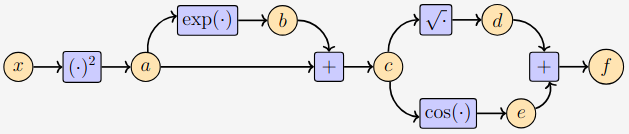
\includegraphics[
            width=\linewidth,
            height=2cm,
            keepaspectratio,
        ]{images/Vector-Calculus/example-auto-diff-comp-graph.png}
        \caption*{
            Computation graph with inputs $x$, function values $f$, and intermediate variables $a, b, c, d, e$.
            \cite{mfml/book/mml/Deisenroth-Faisal-Ong}
        }
    \end{figure}
    \begin{multicols}{6}
    \begin{enumerate}[leftmargin=0.1cm, label={}]
        \item[] $a = x^2$
        \item[] $b = \exp(a)$
        \item[] $c = a+b$
        \item[] $d = \sqrt{c}$
        \item[] $e = \cos(c)$
        \item[] $f = d+e$
    \end{enumerate}
    \end{multicols}
    \begin{multicols}{6}
    \begin{enumerate}[leftmargin=0.1cm, label={}]
        \item[] $\dfrac{\partial a}{\partial x} = 2x$
        \item[] $\dfrac{\partial b}{\partial a} = \exp(a)$
        \item[] $\dfrac{\partial c}{\partial a} = \dfrac{\partial c}{\partial b} = 1$
        \item[] $\dfrac{\partial d}{\partial c} = \dfrac{1}{2\sqrt{c}}$
        \item[] $\dfrac{\partial e}{\partial c} = -\sin(c)$
        \item[] $\dfrac{\partial f}{\partial d} = \dfrac{\partial f}{\partial e} = 1$
    \end{enumerate}
    \end{multicols}
    \begin{multicols}{3}
    \begin{enumerate}[leftmargin=0.1cm, label={}]
        \item[] $
            \dfrac{\partial f}{\partial c}
            = \dfrac{\partial f}{\partial d} \dfrac{\partial d}{\partial c}
            + \dfrac{\partial f}{\partial e} \dfrac{\partial e}{\partial c}
        $
        \item[] $
            \dfrac{\partial f}{\partial a}
            = \dfrac{\partial f}{\partial b} \dfrac{\partial b}{\partial a}
            + \dfrac{\partial f}{\partial c} \dfrac{\partial c}{\partial a}
        $
        \item[]
        $
            \dfrac{\partial f}{\partial b}
            = \dfrac{\partial f}{\partial c} \dfrac{\partial c}{\partial b}
        $
            \hspace{0.2cm}
            \vline
            \hspace{0.2cm}
        $
            \dfrac{\partial f}{\partial x}
            = \dfrac{\partial f}{\partial a} \dfrac{\partial a}{\partial x}
        $
    \end{enumerate}
    \end{multicols}
\end{enumerate}





\section{Taylor Series \& Polynomial}

\begin{enumerate}
    \item
    \begin{definition}[Taylor Series ($T_{\infty}(x)$)]
        For a smooth function $f \in C^{\infty}$, $f : \mbbR \to \mbbR$, the Taylor series of $f$ at $x_0$ is defined as
        $
            f(x) = T_{\infty}(x)
            = \dsum_{k=0}^{\infty} \dfrac{f^{(k)}(x_0)}{k!} (x - x_0)^k
        $
        \hfill \cite{mfml/book/mml/Deisenroth-Faisal-Ong}
        \\
         $f \in C^{\infty}$ means that $f$ is continuously differentiable infinitely many times
         \hfill \cite{mfml/book/mml/Deisenroth-Faisal-Ong}
    \end{definition}
    \begin{enumerate}
        \item
        \begin{definition}[Maclaurin series]
            For $x_0 = 0$, we obtain the \textbf{Maclaurin series} as a special instance of the Taylor series.
            \hfill \cite{mfml/book/mml/Deisenroth-Faisal-Ong}
        \end{definition}

        \item
        \begin{definition}[Analytic]
            If $f (x) = T_{\infty}(x)$, then $f$ is called \textbf{analytic}.
            \hfill \cite{mfml/book/mml/Deisenroth-Faisal-Ong}
        \end{definition}
    \end{enumerate}

    \item
    \begin{definition}[Multivariate Taylor Series]
        We consider a function $f: \mbbR^D \to \mbbR, \bm{x} \mapsto f(\bm{x}), \bm{x} \in \mbbR^D$ that is smooth at $\bm{x}_0$.
        When we define the difference vector $\bm{\delta} := \bm{x} - \bm{x}_0$, the multivariate Taylor series of $f$ at $(\bm{x}_0)$ is defined as
        \hfill \cite{mfml/book/mml/Deisenroth-Faisal-Ong}
        \\
        .\hfill
        $
            f(\bm{x})
            = \dsum_{k=0}^{\infty} \dfrac{D^k_{\bm{x}}\ f(\bm{x}_0)}{k!} \bm{\delta}^k
        $
        \hfill \cite{mfml/book/mml/Deisenroth-Faisal-Ong}
        \\
        where $D^k _{\bm{x}}\ f (\bm{x}_0)$ is the $k$-th (total) derivative of $f$ with respect to $\bm{x}$, evaluated at $\bm{x}_0$.
        \\
        SEE: Outer product
        \hfill \cite{mfml/book/mml/Deisenroth-Faisal-Ong}
    \end{definition}

    \item
    \begin{definition}[Taylor Polynomial ( $T_n(x)$ )]
        The Taylor polynomial of degree $n$ of $f : \mbbR \to \mbbR$ at $x_0$ is defined as
        $
            T_n(x)
            := \dsum_{k=0}^n \dfrac{f^{(k)}(x_0)}{k!} (x - x_0)^k
        $
        \hfill \cite{mfml/book/mml/Deisenroth-Faisal-Ong}
        \\
        where $f ^{(k)}(x_0)$ is the $k$-th derivative of $f$ at $x_0$ (which we assume exists) and $\dfrac{f ^{(k)}(x_0)}{ k!}$ are the coefficients of the polynomial.
        \hfill \cite{mfml/book/mml/Deisenroth-Faisal-Ong}
        \\
        We define $t^0 := 1$ for all $t \in \mbbR$.
        \hfill \cite{mfml/book/mml/Deisenroth-Faisal-Ong}
    \end{definition}
    \begin{enumerate}
        \item In general, a Taylor polynomial of degree $n$ is an \textbf{approximation} of a function, which does not need to be a polynomial.
        The Taylor polynomial is similar to $f$ in a neighborhood around $x_0$.
        Higher-order Taylor polynomials approximate the function $f$ better and more globally.
        \hfill \cite{mfml/book/mml/Deisenroth-Faisal-Ong}

        \item A Taylor polynomial of degree $n$ is an \textbf{exact} representation of a polynomial $f$ of degree $k \leq n$ since all derivatives $f (i)$, $i > k$ vanish.
        \hfill \cite{mfml/book/mml/Deisenroth-Faisal-Ong}
    \end{enumerate}

    \item
    \begin{definition}[Multivariate Taylor Polynomial ( $T_n(\bm{x})$ )]
        The Taylor polynomial of degree $n$ of $f : \mbbR^D \to \mbbR$ at $\bm{x}_0$ is defined as
        $
            T_n(x)
            := \dsum_{k=0}^n \dfrac{D^k_{\bm{x}} f(\bm{x}_0)}{k!} \bm{\delta}^k
        $
        \hfill \cite{mfml/book/mml/Deisenroth-Faisal-Ong}
        \\
        where $D^k _{\bm{x}}\ f (\bm{x}_0)$ is the $k$-th (total) derivative of $f$ with respect to $\bm{x}$, evaluated at $\bm{x}_0$.
        \\
        SEE: Outer product
        \hfill \cite{mfml/book/mml/Deisenroth-Faisal-Ong}
    \end{definition}
\end{enumerate}

















